
\chapter{Preface}
\label{cha:preface}

A central topic in linear algebra is the theory around  linear equations 
\begin{equation} 
\label{p:eq:1}
  A \, x = b
\end{equation}
where $A ∈ ℝ^{m×n}$ is a given matrix and $b ∈ ℝ^m$ is a given vector. Every student of mathematics learns learns to appreciate \emph{Gaussian elimination} which transforms the system~\eqref{p:eq:1}  into an equivalent system  
\begin{displaymath}
  {A}' x = {b}'
\end{displaymath}
that is in row-echelon form. This means that ${A}' ∈ ℝ^{m×n}$ is such that 
  for each $i ∈ \{ 1,\dots , m-1\}$
  \begin{displaymath}
    \min\{ j : {a}'_{ij} \neq 0\} <  \min\{ j : {a}'_{i+1j} \neq 0\},
  \end{displaymath}
see Figure~\ref{fig:8}. 


\begin{figure}
  \centering
 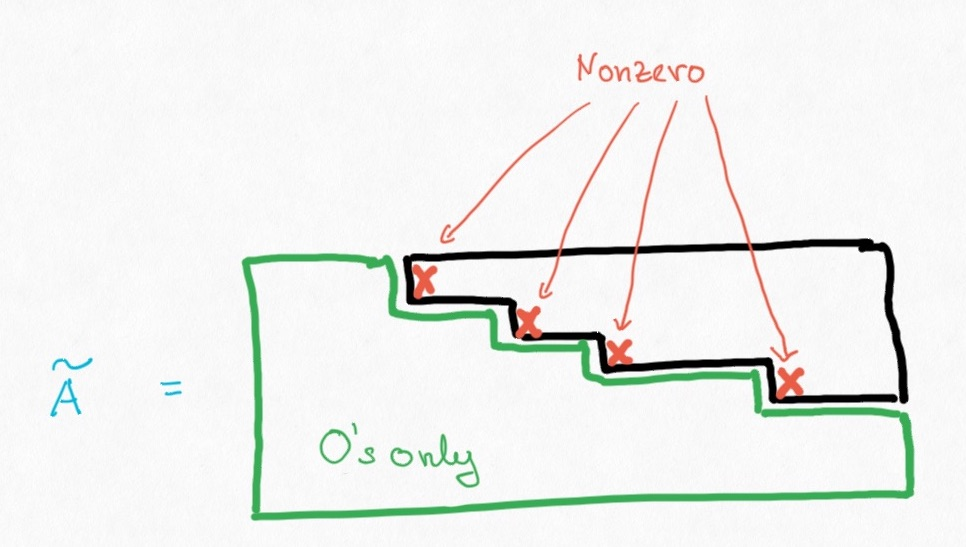
\includegraphics[height=5cm]{figures/RowEchelon.jpg}
  \caption{A schematic image of a matrix in row-echelon form} 
\label{fig:8}
\end{figure}


The system~\eqref{p:eq:1} has a solution if and only if ${b}'$ has only zero's in those components that correspond to the zero-rows of ${A}'$ and a solution is readily computed. In fact, Gaussian elimination also provides an invertible matrix $Q ∈ ℝ^{m ×m}$ such that $Q\cdot A = {A}'$ and $Q \cdot b = {b}'$. If the $i$-th component of ${b}'$ is nonzero and the $i$-th row of ${A}'$ consists of zeros only, then with $q$ being the column vector corresponding to the $i$-th row of $Q$ one has 
\begin{displaymath}
  q^T A = 0 \text{ and } q^Tb \neq 0. 
\end{displaymath}
Thus there is a convenient \emph{certificate} of the fact that \eqref{p:eq:1} is not solvable. 


\begin{theorem}
  \label{thr:8}
  A linear system~\eqref{p:eq:1} is not solvable if and only if there exists a vector $q ∈ ℝ^m$ such that 
  \begin{displaymath}
    q^T A = 0 \text{ and } q^T b \neq 0. 
  \end{displaymath}
\end{theorem}

In this course, we will now also deal with systems of \emph{linear inequalities} 
\begin{equation}
  \label{p:ineq}
  A \,x ≤ b,
\end{equation}
where $A ∈ ℝ^{m × n}$ and $b ∈ ℝ^m$. A \emph{solution} to such a system is a vector $x^* ∈ ℝ^m$ such that
\begin{equation}
  \label{p:sol}
 \text{for each } i=1,\dots,m \quad : \quad   a_{i1} x^*_1 + \cdots + a_{in} x^*_n \leq b_i.  
\end{equation}
If a solution exists, the system~\eqref{p:ineq} is called \emph{feasible} otherwise it is called \emph{infeasible}. 
We will ask analogous questions for  systems of linear inequalities as we did for linear equations. Can we efficiently find a solution of~\eqref{p:ineq}?  Is there a simple certificate to convince somebody of the infeasibility of \eqref{p:ineq}? 

To shed a bit of light on this second question, let us consider a vector $λ ∈ ℝ^m_{≥0}$. If $x^*$ is a solution, then $x^*$ also satisfies the inequality 
\begin{equation}
  \label{p:impli}
  λ^T A \, x ≤ λ^T b.
\end{equation}
If there exists a $λ \in ℝ^m_{≥0}$ such that 
\begin{equation}
  \label{p:Farkas}
  λ^T A = 0^T \text{ and } λ^T b = -1,
\end{equation}
then this $λ$ \emph{certifies} that~\eqref{p:ineq} is infeasible. In the case of infeasibility, can such a $λ≥0$ always be found? Among the many results presented in  this course,  we will show that the answer is ``yes''. 
\begin{theorem}[Farkas' lemma]
  \label{thr:7}
  A system of linear inequalities~\eqref{p:ineq} is infeasible if and only if there exists a $λ ∈ ℝ^m_{≥0}$ such that 
  \begin{displaymath}
    λ^T A = 0 \text{ and } λ^T b = -1.
  \end{displaymath}
\end{theorem}


Central to this course is the \emph{linear programming} or \emph{linear optimization} problem.  There, one is given a system of linear inequalities~\eqref{p:ineq} together with a linear objective function $f(x) = c^Tx$ for some fixed $c ∈ℝ^n$. The task is to solve 
\begin{equation}
  \label{eq:1}
  \max\{ c^Tx : x ∈ ℝ^n, \, Ax \leq b\}, 
\end{equation}
or in other words, to find an $x^* ∈ ℝ^n$ that is a solution of \eqref{p:ineq} such that $c^T x^* ≥ c^T y^*$ for each solution $y^*$ of \eqref{p:ineq}, if such an $x^*$ exists. 
The linear optimization problem is one of the most important types of mathematical optimization problems. It has numerous applications in science and engineering and, in particular, modern fields like \emph{machine learning}.

In this course, we will learn  the theory of linear optimization and develop \emph{efficient algorithms} to solve linear programming problems. This means that we do not content ourselves with an algorithm that is correct, but we want this algorithm to be capable to solve large scale problems within a short time. 

\emph{Efficient algorithms} is a subfield of computational mathematics on its own. Before we begin with our considerations on linear programming, we will have to learn the basics of it. 






\section*{Exercises}

\begin{enumerate}[1)]
\item Provide a certificate as in Theorem~\ref{thr:8} of the unsolvability of the linear equation 
  \begin{displaymath}
    \begin{pmatrix}
      2 & 1 & 0 \\
      5 & 4 & 1 \\
      7 & 5 & 1
    \end{pmatrix} \,
    \begin{pmatrix}
      x_1 \\ x_2 \\ x_3 
    \end{pmatrix} =
    \begin{pmatrix}
      1\\2\\4
    \end{pmatrix}
  \end{displaymath}
\item Show the ``if'' direction of the Farkas' lemma (Theorem~\ref{thr:7}). 
\end{enumerate}



 

%%% Local Variables: 
%%% mode: latex
%%% TeX-master: "lecture"
%%% End: 
